\section{Arrays}

\subsection{Definition}
An \textbf{array} is a data structure that stores elements in \textbf{contiguous blocks of memory}.  
Each element can be accessed directly using its index.

\subsection{Memory Layout}
\begin{figure}[h]
\centering
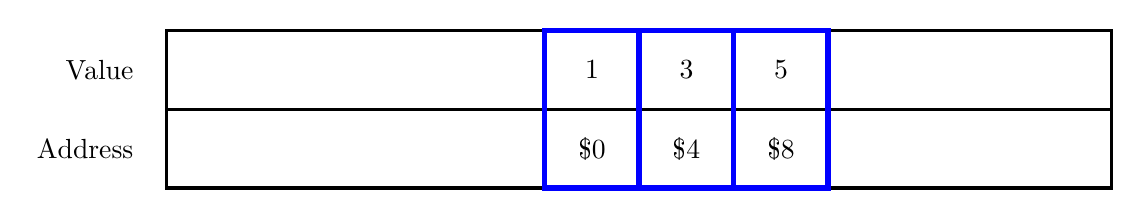
\begin{tikzpicture}[x=1cm,y=1cm]

% --- Geometry settings ---
\def\W{12}        % total width of the big memory block
\def\H{2}         % total height (2 rows)
\def\cellW{1.2}   % width of each cell in the highlighted region
\def\nCells{3}
\def\hiX{4.8}     % x-position where the highlighted region starts (centered-ish)

% --- Outer "RAM block" rectangle and the row divider ---
\draw[line width=1.2pt] (0,0) rectangle (\W,\H);
\draw[line width=1.2pt] (0,1) -- (\W,1);

% --- Labels on the left (no overlap) ---
\node[anchor=east] at (-0.3,1.5) {Value};
\node[anchor=east] at (-0.3,0.5) {Address};

% --- Highlighted region: contiguous cells spanning both rows ---
% Outer highlight frame
\draw[draw=blue, line width=2pt] (\hiX,0) rectangle ({\hiX+\nCells*\cellW},\H);

% Internal vertical dividers for each cell
\foreach \i in {1,...,2} {
  \draw[draw=blue, line width=2pt]
    ({\hiX+\i*\cellW},0) -- ({\hiX+\i*\cellW},\H);
}

% --- Text inside cells ---
\node at ({\hiX+0.5*\cellW},1.5) {1};
\node at ({\hiX+1.5*\cellW},1.5) {3};
\node at ({\hiX+2.5*\cellW},1.5) {5};

\node at ({\hiX+0.5*\cellW},0.5) {\$0};
\node at ({\hiX+1.5*\cellW},0.5) {\$4};
\node at ({\hiX+2.5*\cellW},0.5) {\$8};

\end{tikzpicture}
\caption{Arrays are stored in contiguous blocks of memory}
\end{figure}


Because memory is contiguous, the address of any element can be computed in constant time:
\[
\text{address}(i) = \text{base} + i \cdot \text{sizeof(element)}
\]

\subsection{Types of Arrays}

\textbf{Static Arrays}
\begin{itemize}
  \item Fixed size determined at creation time
  \item Stored in one continuous block of memory
  \item Cannot grow or shrink
  \item Memory-efficient (no resizing overhead)
\end{itemize}
\textbf{Dynamic Arrays}
\begin{itemize}
  \item Automatically resize when capacity is reached
  \item Implemented using an underlying static array
  \item When full:
    \begin{itemize}
      \item A new array (usually 2× larger) is allocated
      \item All elements are copied to the new array
      \item Old array is deallocated
    \end{itemize}
  \item Appending is \textbf{amortized} to $O(1)$
\end{itemize}

\subsection{Time Complexity}

\begin{center}
\begin{tabular}{l c}
\toprule
\textbf{Operation} & \textbf{Time Complexity} \\
\midrule
Read by index & $O(1)$ \\
Write at end (append) & $O(1)$ \\
Insert at beginning & $O(n)$ \\
Insert in middle & $O(n)$ \\
Insert at end & $O(1)$ \\
Remove from beginning & $O(n)$ \\
Remove from middle & $O(n)$ \\
Remove at end & $O(1)$ \\
\bottomrule
\end{tabular}
\end{center}

\subsection{Why Some Operations Are Slow}
Inserting or removing elements at the beginning or middle of an array requires shifting all subsequent elements to preserve contiguous memory, which is $O(n)$.